% testing.tex
\chapter{Testing}

\section{Test Strategy}
Video demonstration of the app will be provided to show the app in action, this will provide a complete overview of the app and its features. This is my acceptance testing as it will show the app working and meeting the original requirements.

The primary testing strategy for my backend project would be Unit testing to see if all the smaller components of my app work as intended. Django provide its own testing framework built on top of Python's unittest module. I will be using this to test my models and the methods within them, as well as the utility functions I have created in my app. Normal, boundary and edge cases will be tested where applicable. In addition, the PostgreSQL database will also be shown in a video.

For the API endpoints I will be using REST client provided by Visual Studio Code to make HTTP requests to the server and compare the result with my anticipated result. I will be doing this rather than using Django's own testing framework because I want to model real world usage of my app by making legitimate HTTP requests to actually modify application.

For my frontend Interface, I will be will be testing the app manually by interacting with the components to see if the app behaves as expected. This is also act as my integration testing as I will be testing the app as a whole - frontend depends on the backend.

\subsection{Unit Testing}
\subsubsection{User}
Here are the unit tests I have written for the User model in my app, the purpose of the tests are evident from the name of the tests.:
\begin{minted}{python3}
from django.test import TestCase
from django.core.exceptions import ValidationError
from Users.models import MyUser
from .utils import validate_email, clean_email, hash_password, verify_password

from django.test import TestCase
from .utils import hash_password, verify_password, validate_email, clean_email


class UtilityFunctionTests(TestCase):

    def test_hash_password(self):
        password = "testpassword123"
        hashed_password = hash_password(password)
        self.assertIsInstance(hashed_password, str)
        self.assertTrue(":" in hashed_password)

    def test_verify_password(self):
        password = "testpassword123"
        hashed_password = hash_password(password)
        self.assertTrue(verify_password(password, hashed_password))

    def test_verify_password_incorrect(self):
        password = "testpassword123"
        incorrect_password = "wrongpassword"
        hashed_password = hash_password(password)
        self.assertFalse(verify_password(incorrect_password, hashed_password))

    def test_validate_email_valid(self):
        valid_email = "test@test.com"
        self.assertTrue(validate_email(valid_email))

    def test_validate_email_invalid(self):
        invalid_email = "not-an-email"
        self.assertFalse(validate_email(invalid_email))

    def test_clean_email_valid(self):
        valid_email = "test@test.com"
        self.assertEqual(clean_email(valid_email), valid_email)

    def test_clean_email_all_caps(self):
        test_email = "TEST@TEST.COM"
        self.assertEqual(clean_email(test_email), test_email.lower())

    def test_clean_email_with_extra_characters(self):
        valid_email = "      test@test.com  "
        self.assertEqual(clean_email(valid_email), "test@test.com")


class MyUserModelTests(TestCase):

    def test_create_user(self):
        email = "test@test.com"
        password = "password"
        user: MyUser = MyUser.objects.create_user(email=email, password=password)
        self.assertEqual(user.email, email)
        self.assertTrue(user.check_password(password))

    def test_create_user_invalid_email(self):
        email = "not-an-email"
        password = "password"
        with self.assertRaises(ValueError):
            MyUser.objects.create_user(email=email, password=password)
\end{minted}

\begin{figure}[H]
    \centering
    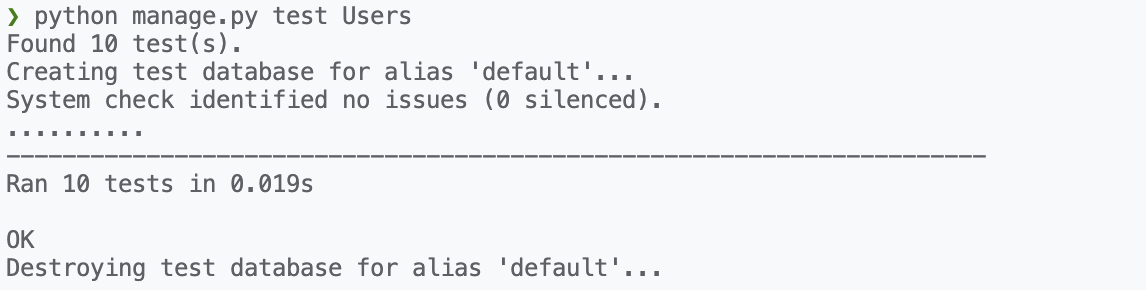
\includegraphics[width=\textwidth]{Assets/users_test_result.png}
    \caption{Unit Test Result for User App in Django}
    \label{fig:unit_test_user}
\end{figure}


\subsubsection{Journal}
Here are the unit tests I have written for the Journal model in my app:

\begin{minted}{python3}
    from django.test import TestCase
    from .models import Journal, Entry
    from Users.models import MyUser
    
    
    class JournalModelTests(TestCase):
        def setUp(self):
            self.user = MyUser.objects.create_user(
                email="test@test.com", password="password"
            )
    
        # test if an entry asssociated with the user is created automatically using a signal
        def test_create_journal(self):
            journal = Journal.objects.get(user_id=self.user)
            self.assertEqual(journal.user_id, self.user)
            self.assertEqual(journal.get_all_entries().count(), 0)
    
        def test_create_entry(self):
            journal = Journal.objects.get(user_id=self.user)
            entry = Entry.objects.create(journal_id=journal, content="first entry")
            self.assertEqual(entry.journal_id, journal)
            self.assertEqual(journal.get_all_entries().count(), 1)
    
        def test_get_all_entries(self):
            journal = Journal.objects.get(user_id=self.user)
            entry1 = Entry.objects.create(journal_id=journal, content="first entry")
            entry2 = Entry.objects.create(journal_id=journal, content="second entry")
            self.assertEqual(journal.get_all_entries().count(), 2)
\end{minted}

\begin{figure}[H]
    \centering
    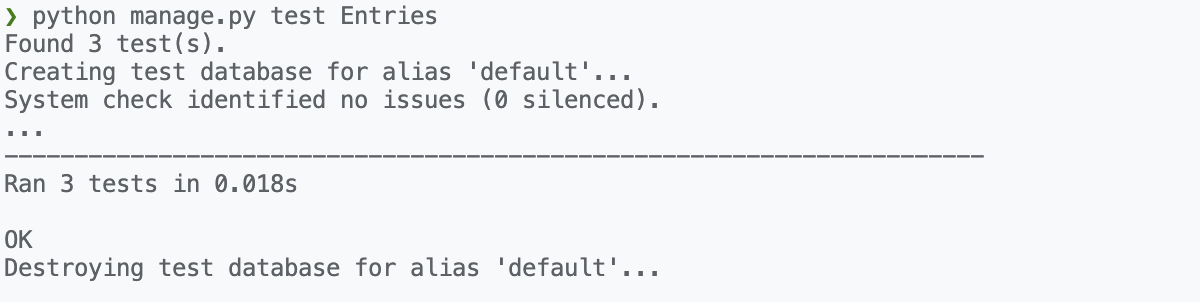
\includegraphics[width=\textwidth]{Assets/entries_test_result.png}
    \caption{Unit Test Result for Entries App in Django}
    \label{fig:unit_test_entries}
\end{figure}

\section{Endpoints}
To model real world usage, I will be making HTTP requests to the server and compare the result with my anticipated result. Here are a list of views created in my app:

\begin{minted}{python3}
    # from entries/urls.py
    urlpatterns = [
        re_path("sample/", views.sampleEntry, name="sample entry"),
        re_path("testUser/", views.test_user, name="test user"),
        re_path("getEntries/", views.get_all_entries, name="get all entries"),
        re_path("createEntry/", views.create_entry, name="create entry"),
        re_path(
            "getScheduledUsers/",
            views.get_daily_scheduled_email_users,
            name="get scheduled email users",
        ),
        re_path("deleteEntry/", views.delete_entry, name="delete entry"),
        re_path(
            "getJournalStatistics/",
            views.get_journal_statistics,
            name="get entry statistics",
        ),
    ]
\end{minted}


\begin{minted}{python3}
    # from users/urls.py
    urlpatterns = [
        re_path("register/", views.register_view, name="api_register"),
        re_path("login/", views.login_view, name="api_login"),
        re_path("logout/", views.logout_view, name="api_logout"),
        re_path("test_user/", views.test_user, name="test_user"),
        # re_path("update_email_prompt/", views.update_email_prompt, name="email_prompt"),
        # path("session/", views.session_view, name="api_session"),
    ]
\end{minted}
\subsection{Endpoint tests with Rest Client}
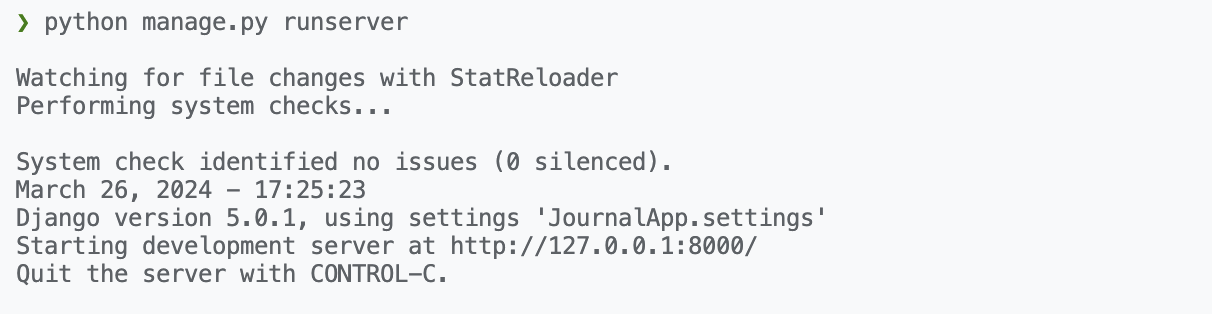
\includegraphics[width=\textwidth]{Assets/django_running.png}

\subsubsection{Once the server is running, I began to make requests, Appendix \ref{} for the results}
\subsection{Test Cases Summary}

\begin{table}[H]
\centering
\begin{tabular}{|l|l|l|}
\hline
\textbf{Test Case}                             & \textbf{Outcome} & \textbf{Figure Reference} \\ \hline
Register a new user that already exists        & Successful      & Fig.~\ref{fig:request_register_already_exist}, \ref{fig:response_register_already_exist} \\ \hline
Register a new user that does not exist        & Successful      & Fig.~\ref{fig:request_register_new_user}, \ref{fig:response_register_new_user} \\ \hline
Register a new user with an invalid email      & Successful      & Fig.~\ref{fig:request_register_invalid_email}, \ref{fig:response_register_invalid_email} \\ \hline
Login with a valid user                        & Successful      & Fig.~\ref{fig:request_login_sucessful}, \ref{fig:response_login_sucessful} \\ \hline
Login with an invalid user                     & Successful      & Fig.~\ref{fig:request_login_invalid_user}, \ref{fig:response_login_invalid_user} \\ \hline
Login with an invalid password                 & Successful      & Fig.~\ref{fig:request_login_invalid_password}, \ref{fig:response_login_invalid_password} \\ \hline
Login with an invalid email                    & Successful      & Fig.~\ref{fig:request_login_invalid_email}, \ref{fig:response_login_invalid_email} \\ \hline
Test user authentication with a valid token    & Successful      & Fig.~\ref{fig:request_test_user_authtoken}, \ref{fig:response_test_user_authtoken} \\ \hline
Test user authentication with an invalid token & Successful      & Fig.~\ref{fig:request_test_user_authtoken_invalid}, \ref{fig:response_test_user_authtoken_invalid} \\ \hline
Get samples of entries                                   & Successful      & Fig.~\ref{fig:request_get_samples}, \ref{fig:response_get_samples} \\ \hline
Test user in entry app                         & Successful      & Fig.~\ref{fig:request_test_user_entry}, \ref{fig:response_test_user_entry} \\ \hline
Create a new entry                             & Successful      & Fig.~\ref{fig:request_create_new_entry}, \ref{fig:response_create_new_entry} \\ \hline
Get entries                                   & Successful      & Fig.~\ref{fig:request_get_entry}, \ref{fig:response_get_entry} \\ \hline
Delete entries with an invalid id             & Successful      & Fig.~\ref{fig:request_delete_entry_invalid}, \ref{fig:response_delete_entry_invalid} \\ \hline
Delete an entyr with a valid id                & Successful      & Fig.~\ref{fig:request_delete_entry_valid}, \ref{fig:response_delete_entry_valid} \\ \hline
Get journal statistics                         & Successful      & Fig.~\ref{fig:request_get_journal_statistics}, \ref{fig:response_get_journal_statistics} \\ \hline
\end{tabular}
\caption{Summary of API Test Cases, Outcomes, and Figure References}
\label{table:test_cases_summary}
\end{table}

\newpage

\section{Frontend Interface}    
See test videos for the frontend interface being interacted with.

\section{Testing Video}
The video demonstrates the app in action, showing the app working and meeting the original requirements. The video can be found at the following link: \url{https://drive.google.com/drive/folders/1aORi1Iy9CklbfWv4FY6oDLnTgXSax8Gc?usp=sharing}
\begin{figure}[H]
    \centering
    
\includegraphics[width=\textwidth]{Assets/qr_videos.png}
    \caption{Testing Videos}
    \label{fig:testing_video}
\end{figure}

\section{System Tests}
Comparing my current app against my original requirements:
\begin{table}[H]
    \centering
    \begin{tabular}{|l|p{8cm}|p{4cm}|}  
    \hline
    \textbf{ID} & \textbf{Requirement Description}& \textbf{Has Been Met} \\ \hline
    1.1 & Design data models for users, journal entries, with relationships defined. & Yes\\ \hline
    
    1.2 & Have an effective way to check the submitted user information, journal entries, and related data before stored in the database, ensuring data stored are in the required format. & Yes \\ \hline
    
    1.3 & Have a way to generate statistics of the user's journaling habits, such as the most active month of the user, average entries made per week, etc. & Yes \\ \hline
    
    2.1 & Develop API endpoints with functionalities implemented to handle user authentication (login and registration) and other core endpoints that drives the journal app as a whole & Yes\\ \hline
    
    2.2 & Features for secure password storage(salting and hashing) and and authenticate; token generation for session management.& Yes\\ \hline
    
    3.1 & Ensure all API endpoints are secured and accessible only to authenticated users, using tokens or similar mechanisms for session management.& Yes \\ \hline
    
    3.2 & Ensure smooth and spontaneous communication with the frontend. & Yes\\ \hline
    4.1 & Design the Backend with the room for more functionalities & Yes \\ \hline
    
    \end{tabular}
    \caption{Backend Requirements for Journal App}
\end{table}

\begin{table}[H]
    \centering
    \begin{tabular}{|l|p{8cm}|p{4cm}|}
    \hline
    \textbf{ID} & \textbf{Requirement Description} & \textbf{Has Been Met}\\ \hline
    1.1 & Develop a login page to authenticate users, include forms for user input and dynamically provide error/feedback when necessary. & Yes \\ \hline
    
    1.2 & Implement a registration page enabling new users to create an account, take in input for email, password, last name, first name and interact/update backend. Provide feedback to the user after submission. & Yes\\ \hline
    
    1.3 & Develop a place where the user can see details about themselves ie their personal information and journal statistics & Yes\\ \hline
    
    2.1 & Create a page for users to compose new journal entries. Input parameters are title and content of the entry. Interact with the corresponding endpoint and provide feedback to the user.& Yes\\ \hline
    
    2.2 & Design a retrieve journal page that lists all the user’s entries, with options for sorting the entries in ascending or descending order based on creation date or other criteria in an efficient way. & Yes\\ \hline
    
    3.1 & Implement navigation bar that adjusts its visibility of options based on the user's login status. & Yes\\ \hline
    
    4.1 & Utilize state management techniques to keep the user logged in across different pages, preserving session information securely. & Yes\\ \hline
    
    4.2 & Handle fetching, posting, and updating data through JSON responses from the backend. & Yes \\ \hline
\end{tabular}
\caption{Frontend Requirements for Journal App}
\end{table}
    